% This is samplepaper.tex, a sample chapter demonstrating the
% LLNCS macro package for Springer Computer Science proceedings;
% Version 2.20 of 2017/10/04
%
\documentclass[runningheads]{llncs}
%
\usepackage{graphicx}
% Used for displaying a sample figure. If possible, figure files should
% be included in EPS format.
%
% If you use the hyperref package, please uncomment the following line
% to display URLs in blue roman font according to Springer's eBook style:
% \renewcommand\UrlFont{\color{blue}\rmfamily}

\begin{document}
%
\title{Subtle Gestures with the J!NS MEME}
%
%\titlerunning{Abbreviated paper title}
% If the paper title is too long for the running head, you can set
% an abbreviated paper title here
%
\author{Thomas Bartel \and
Florian Bossert \and
Sajjad Ahmad}
%
% TODO should we use 'et al.' here? ~FB
\authorrunning{T. Bartel \and F. Bossert \and S. Ahmad}
% First names are abbreviated in the running head.
% If there are more than two authors, 'et al.' is used.
%
\institute{Karlsruhe Institute of Technology, Karlsruhe, Germany}
%
\maketitle              % typeset the header of the contribution
%
\begin{abstract}
The abstract should briefly summarize the contents of the paper in
15--250 words.

\keywords{First keyword  \and Second keyword \and Another keyword.}
\end{abstract}
%
%
%
\section{Introduction}
\subsection{A Subsection Sample}
Please note that the first paragraph of a section or subsection is
not indented. The first paragraph that follows a table, figure,
equation etc. does not need an indent, either.

Subsequent paragraphs, however, are indented.

% As a reference, maybe useful later
Current smartglasses:
Smartglasses with cameras: Spectacles by Snap Inc. https://www.spectacles.com/
Smartglasses with EOG sensors: J!ns Meme by J!ns (website currently only in Japanese): https://jins-meme.com/

% Assigned to FB
\section{Related Work}
[Insert an introduction here]

\subsection{Face Interaction}
Detecting finger tapping on the body using acoustic sensing \cite{10.1145/1753326.1753394}.
Optical tracking system with infrared markers on fingers \cite{10.1145/2556288.2556984}.
Exploring touch interaction by placing electrodes around the ear \cite{10.1145/2468356.2468592}.
Exploring tooth click gestures \cite{10.1145/2935334.2935389}.
Eyelid gestures \cite{10.5555/2788890.2788938}.
Finger sensing IMUs \cite{10.1145/2858036.2858466}.
Hand sensing IMUs \cite{10.1145/2984511.2984582}.
Gesture recognition using wrist band \cite{10.1145/3274783.3274854}.
Tracking tongue movements with touch sensors \cite{10.1145/3311823.3311831}.
\subsection{Applications for Wearable Sensing}
Tracking eating episodes \cite{10.1145/3130902}.
Sensors in shoes for tracking exercises \cite{10.1145/3174910.3174938}.
Using hand gestures to control TV with wrist band \cite{10.1145/2641248.2641359}.
Jump performance analysis \cite{10.1145/2753509.2753512}.
Monitoring drinking with wrist-worn inertial sensors \cite{10.1145/3267242.3267253}.
\subsection{EOG Sensing and Subtle Interaction}
EOG attached to over-ear head phones \cite{10.1145/1125451.1125655}.
EOG attached to in-ear head phones \cite{10.1145/2493988.2494329}.
Demonstration of EOG sensors for eye-tracking \cite{10.1145/1520340.1520468}.
Commercial EOG glasses for activity recognition, passively \cite{10.1145/2638728.2638795}.
KissGlass for passively sensing context, not for deliberate subtle interactions \cite{10.1145/3384657.3384801}.
Defining subtlety \cite{10.1145/3290605.3300648}. 
Itchy Nose \cite{10.1145/3123021.3123060}.
% Should this one even be in the Related Work category or just mentioned in Analysis?
Itchy Nose tool for automating personalization \cite{10.1145/3174910.3174953}.

% Assigned to FB
\section{Analysis}
What was our workflow?

Which gestures did we choose?

How does the J!ns Meme work and how do we use it?

What data do we collect, how and why?

% Assigned to TB
\section{Implementation}
\subsection{A Subsection Sample}
Please note that the first paragraph of a section or subsection is
not indented. The first paragraph that follows a table, figure,
equation etc. does not need an indent, either.

Subsequent paragraphs, however, are indented.

% Assinged to SA
\section{Results}
\subsection{A Subsection Sample}
Please note that the first paragraph of a section or subsection is
not indented. The first paragraph that follows a table, figure,
equation etc. does not need an indent, either.

Subsequent paragraphs, however, are indented.

% Assigned to TB
\section{Discussion}
\subsection{A Subsection Sample}
Please note that the first paragraph of a section or subsection is
not indented. The first paragraph that follows a table, figure,
equation etc. does not need an indent, either.

Subsequent paragraphs, however, are indented.

\section{Future Work}
\subsection{A Subsection Sample}
Please note that the first paragraph of a section or subsection is
not indented. The first paragraph that follows a table, figure,
equation etc. does not need an indent, either.

Subsequent paragraphs, however, are indented.

\section{First Section}
\subsection{A Subsection Sample}
Please note that the first paragraph of a section or subsection is
not indented. The first paragraph that follows a table, figure,
equation etc. does not need an indent, either.

Subsequent paragraphs, however, are indented.

\subsubsection{Sample Heading (Third Level)} Only two levels of
headings should be numbered. Lower level headings remain unnumbered;
they are formatted as run-in headings.

\paragraph{Sample Heading (Fourth Level)}
The contribution should contain no more than four levels of
headings. Table~\ref{tab1} gives a summary of all heading levels.

\begin{table}
\caption{Table captions should be placed above the
tables.}\label{tab1}
\begin{tabular}{|l|l|l|}
\hline
Heading level &  Example & Font size and style\\
\hline
Title (centered) &  {\Large\bfseries Lecture Notes} & 14 point, bold\\
1st-level heading &  {\large\bfseries 1 Introduction} & 12 point, bold\\
2nd-level heading & {\bfseries 2.1 Printing Area} & 10 point, bold\\
3rd-level heading & {\bfseries Run-in Heading in Bold.} Text follows & 10 point, bold\\
4th-level heading & {\itshape Lowest Level Heading.} Text follows & 10 point, italic\\
\hline
\end{tabular}
\end{table}


\noindent Displayed equations are centered and set on a separate
line.
\begin{equation}
x + y = z
\end{equation}
Please try to avoid rasterized images for line-art diagrams and
schemas. Whenever possible, use vector graphics instead (see
Fig.~\ref{fig1}).

\begin{figure}
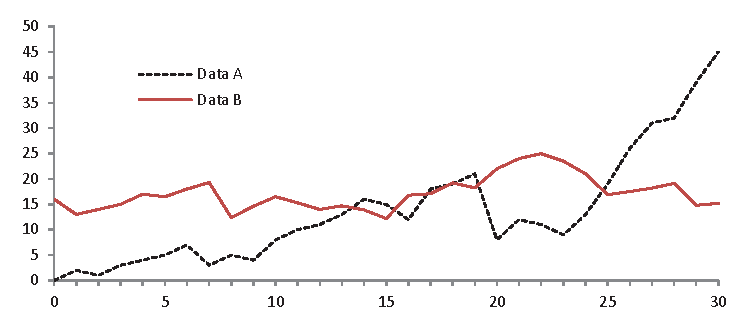
\includegraphics[width=\textwidth]{fig1.eps}
\caption{A figure caption is always placed below the illustration.
Please note that short captions are centered, while long ones are
justified by the macro package automatically.} \label{fig1}
\end{figure}

\begin{theorem}
This is a sample theorem. The run-in heading is set in bold, while
the following text appears in italics. Definitions, lemmas,
propositions, and corollaries are styled the same way.
\end{theorem}
%
% the environments 'definition', 'lemma', 'proposition', 'corollary',
% 'remark', and 'example' are defined in the LLNCS documentclass as well.
%
\begin{proof}
Proofs, examples, and remarks have the initial word in italics,
while the following text appears in normal font.
\end{proof}
For citations of references, we prefer the use of square brackets
and consecutive numbers. Citations using labels or the author/year
convention are also acceptable. The following bibliography provides
a sample reference list with entries for journal
% articles~\cite{ref_article1}, an LNCS chapter~\cite{ref_lncs1}, a
% book~\cite{ref_book1}, proceedings without editors~\cite{ref_proc1},
% and a homepage~\cite{ref_url1}. Multiple citations are grouped
% \cite{ref_article1,ref_lncs1,ref_book1},
% \cite{ref_article1,ref_book1,ref_proc1,ref_url1}.
%
% ---- Bibliography ----
%
% BibTeX users should specify bibliography style 'splncs04'.
% References will then be sorted and formatted in the correct style.
%
\bibliographystyle{splncs04}
\bibliography{mybibliography}
%
\end{document}
